\setcounter{page}{1}
\section*{Zielsetzung}
Der Versuch $V46$ verwendet den \emph{Faraday-Effekt}, um die \emph{effektive Masse} von
Galliumarsenid zu bestimmen. Hierzu werden eine undotierte und zwei n-dotierte
Formen des Halbleiters verwendet.

\section{Theorie}
Zu Beginn wird die Verwendung einer effektiven Masse motiviert.
Bevor der Faraday-Effekt beschrieben wird, wird das Phänomen der zirkularen
Doppelbrechung erläutert.

\subsection{Effektive Masse}\label{sec:effektive_masse}
 Bänder eines kristalls sind meist in einer komplexen Bandstruktur angeordnet.
Hierdurch ist eine exakte mathemaische Beschreibung meist schwierig und bedarf
Approximationen. Vorteilhafterweise beschreiben die verwendeten Näherung oftmals
die auftretenden physikalischen Phänomene sehr gut. Bei Halbleitern ist eine
dieser Approximationen, die Betrachtung des Leitungsbandes um das Minium herum.
In der Umgebung um das Minimum kann die Energie des Bandes $\varepsilon$
in Abhängigkeit mit dem Wellenzahlvektor $\vec{k}$ genährt werden als:
\begin{equation}
  \label{eq:gleichung_energie}
  \varepsilon(\vec{k})=\varepsilon(0) + \frac{1}{2}\sum_{i=1}^3 \left.\frac{\partial^2 \varepsilon}{\partial k_i^2}\right|_{k=0}k_i^2 + \mathcal{O}(k^3).
\end{equation}
Dieser Term eröffnet die Einführung der effektiven Masse
\begin{equation}
  \label{eq:effetive_masse}
  m^{*}_i := \frac{\hbar^2}{\left.\frac{\partial^2 \varepsilon}{\partial k_i^2}\right|_{k=0}}.
\end{equation}
Der Vorteil in der Verwendung der effektiven Massse liegt in der Tatsache das
die Definition \eqref{eq:effetive_masse} die Periodiztät des  Kristallpotentials
$V(\vec{r})$ mitberücksichtigt. Somit kann der Hamilton Operator für ein Kristallelektron,
mit Hilfe der effektiven Masse, in einen Hamilton Operator für ein freies
Teilchen überführt werden:
\begin{equation*}
  \hat{H}:\quad \frac{\hbar^2}{2\map{m_e}}\nabla^2 + V(\vec{r}) \quad \rightarrow \quad   \frac{\hbar^2}{2m^*}\nabla^2
\end{equation*}
Ein weiterer Vorteil in der Beschreibung Dynamik mit der effektiven Massse ist,
dass bei anlegen eines externen elektrischen und magnetischen Feldes,
vorrausgesetzt es ist klein, das eine klassiche Newtonsche Betrachtung möglich ist.
Diese Beschaffenheit wird insbesondere im übernächsten Kapitel von nutzen sein.
\subsection{Zirkulare Doppelbrechung}
Wird die Polarisationsebene von linear polarisiertes Licht $E(z)$ bei der Propegation
durch einen Kristall (der Länge $L$) gedreht, wird von zirkularer Doppelbrechung gesprochen (vgl. Abb. \ref{fig:zirkulare_doppelbrechung}).
\begin{figure}
\centering
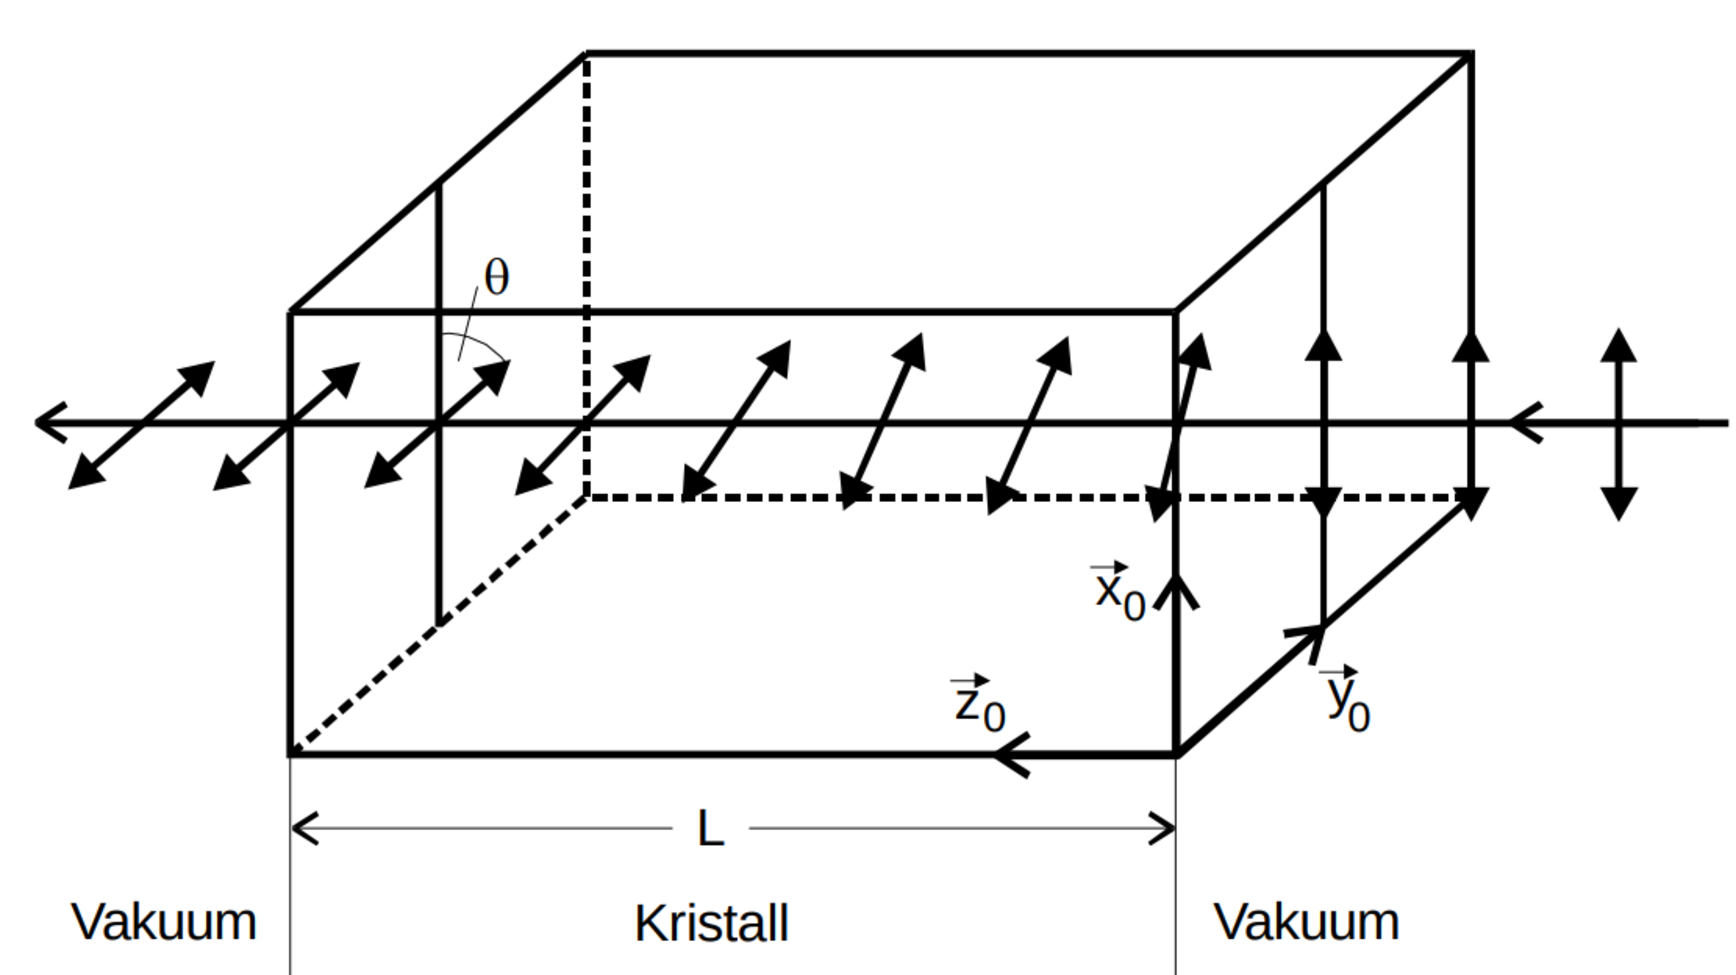
\includegraphics[width=0.5\linewidth]{./content/images/drehung_polarisationsebene.pdf}
\caption{Schmeatische Darstellung von zirkularer Doppelbrechung\cite{glan_thompson_prisma}.}
\label{fig:zirkulare_doppelbrechung}
\end{figure}
Phänomenologisch erklären lässt sich der Effekt unter der Annahme das sich im
Kristall die Phasengeschwindigkeit für links- und rechtszirkular polarisiertes
Licht $E\ua{L}, E\ua{R}$ unterscheiden. Diese Eigenschaft wirkt sich auf die Polarisationsebene
von linear polarisierten Licht aus, weil solches durch eine Linearkombination
von links- und rechtszirkularen Anteilen dargestellt werden kann:
\begin{equation}
  \label{eq:superpos_linear}
\vec{E}(z) = \frac{1}{2}( \vec{E}\ua{R}(z) + \vec{E}\ua{L}(z)), \quad k\ua{R}\neq k\ua{L}
\end{equation}
Wobei die links- und rechtszirkularen definiert sind als
\begin{align}
  \label{eq:def_rechts_links}
  \begin{aligned}
  \vec{E}\ua{R}(z) &= \left(E_0 \vec{x}_0 - \map{i}E_0\vec{y}_0\right)\exp\left(\map{i}{k}\ua{R}z\right)\\
  \vec{E}\ua{L}(z) &= \left(E_0 \vec{x}_0 + \map{i}E_0\vec{y}_0\right)\exp\left(\map{i}{k}\ua{L}z\right)
\end{aligned}
\end{align}
Die Defintionen \eqref{eq:def_rechts_links} werden in die Gleichung \eqref{eq:superpos_linear}
eingesetzt. Zusätzlich werden die Winkel
\begin{align}
  \label{eq:winkel}
  \begin{aligned}
    \Psi&:=\frac{L}{2}(k\ua{R}+k\ua{L}) \\
    \vartheta &:= \frac{L}{2}(k\ua{R}-k\ua{L}) \overset{k_i=\frac{n_i\omega}{\map{c_0}}}{=} \frac{L\omega}{2\map{c_0}}\left(n\ua{R}-n\ua{L}\right)
\end{aligned}
\end{align}
eingeführt, wobei $n$ der jeweilige Brechungsindex ist.
Nach ein wenig Rechnung (nachlesbar in Quelle \cite{anleitungv46}) ergibt sich ein
Ausdruck für das aus dem Kristall austredene Licht:
\begin{equation*}
  \vec{E}(L)=E_0 \exp(\map{i}\Psi)\left(\cos(\vartheta) \vec{x}_0 + \sin(\vartheta)\vec{y}_0\right)
\end{equation*}

Präziser beschrieben werden kann die zirkulare Doppelbrechung durch induzierte
Dipole im Kristall. Die Dipole erzeugen eine Polarisation $\vec{P}$ des Krirtalls,
die für kleine elektrische Felder geschrieben werden kann als
\begin{equation*}
\vec{P}=\varepsilon_0\chi\vec{E}.
\end{equation*}
Hierbei repärsentiert $\varepsilon_0$ die Influenzkonstante und $\chi$ die
\emph{dielektrische Suszeptbilität}, welche in anistropen Kristallen als
Tensor $\tens{\chi}$ geschrieben wird. Doppelbrechung entsteht genau dann, wenn
ein Kristall anistrope Eigenschaften besitzt. Der Beweis dieser Behauptung wird
im folgenden skiziert. Hierzu wird die folgenden dielektrische Suszeptbilität
 $\tens{\chi}$ betrachtet:
\begin{equation}
  \label{eq:chi_tens_example}
  \tens{\chi}=\begin{pmatrix} \chi\ua{xx} & \map{i}\chi\ua{xy} & 0 \\ -\map{i}\chi\ua{yx} & \chi\ua{xx} & 0 \\ 0 & 0 & \chi\ua{zz} \end{pmatrix}.
\end{equation}
Propagiert ein elektrisches Feld durch Matrie so ändert sich das Feld gemäß:
\begin{equation}
  \label{eq:e_feld_in_materie}
  \vec{D}=\varepsilon_0\left(1+\tens{\chi}\right)\vec{E}.
\end{equation}
Wird nun die Gleichung \eqref{eq:e_feld_in_materie} mit \eqref{eq:chi_tens_example}
in die homogene Wellengleichung
\begin{equation*}
  \Box \vec{D} = 0
\end{equation*}
eingesetzt, ergbit sich nach einer etwas längeren Rechnung (vgl. Quelle \cite{anleitungv46}),
dass die Drehung der Polarisationsebene $\vartheta$ gegeben ist durch:
\begin{equation}
  \label{eq:drehung_mit_chi}
  \vartheta \approx \frac{L\omega}{2\map{c_0}}\frac{1}{\sqrt{1+\chi\ua{xx}}}\chi{xy}\approx\frac{L\omega}{2\map{c_0}n}\chi\ua{xy}.
\end{equation}
Bei der Herleitung der Gleichung \eqref{eq:drehung_mit_chi} wurde unter anderem Angenommen,
dass sich die Welle in $z$-Richtung ausbreitet, $\vec{k}=k\vec{z}_0$.
\subsection{Faraday-Effekt}
Der Faraday-Effekt beschreibt die Eigenschaft, dass ein optisch
Medium durch ein externes Magnetfeld Nebendiagnonalen im ielektrische Suszeptbilitättensor
erhält. Hierdurch wird die Polarisationsebene eines, zum Magnetfeld parallel
einfallenden, Lichtfeldes $\vec{E}$ gedreht. Das Phänomen kann präziser erfasst werden,
durch die Betrachtung von gebunden Elektronen im Magnetfeld $\vec{B}$, welche
zusätzlich durch ein elektrisches Feld (verursacht durch die Lichtwelle) gestört wird.
\begin{equation}
  \label{eq:klassische_Bewegungsgleichung}
  m\ddot{\vec{r}}+K\vec{r}=-\map{e}\vec{E}(\vec{r})_0-\map{e}\dot{\vec{r}}\times\vec{B}
\end{equation}
Der Vektor $\vec{r}$ bezeichnet die Auslenkung des Elektrons aus der Gleichgewichtslage,
die Konstante $K$ repärsentiert die Bindung des Elektrons an seine Umgebung, die Elementarladung
ist gegeben durch $\map{e_0}$ und die Feldstärke der einfallenden Lichtwelle
wird durch $\vec{E}$ widergespiegelt.
Unter der Annahme der von quasifreien Ladungsträger kann
aus der Differntialgleichung \eqref{eq:klassische_Bewegungsgleichung} ein Ausdruck
für Drehwinkel der Polarisationsebene $\vartheta$ generiert weren (siehe hierzu Quelle \cite{anleitungv46}):
\begin{equation}
  \label{eq:drehwinkel}
  \frac{\vartheta}{L}\approx \frac{\map{e}^3\lambda^2 NB}{8\pi^2\varepsilon_0\map{c_0}^3}\frac{1}{m^2} = \frac{\map{e}^3\lambda^2 NB}{8\pi^2\varepsilon_0\map{c_0}^3}\frac{1}{m^{*2}}
\end{equation}
Die Ersetzung von $m$ durch $m^*$ ist durch die in Abschnitt \ref{sec:effektive_masse}
besprochene Eigenschaft der effektiven Masse gerechtfertigt. Der Drehwinkel $\vartheta$ hängt somit
mit der Ladungsträgerzahl $N$ und dem Magnetfeldstärke $B$ zusammen.
